% ****** Start of file apssamp.tex ******
%
%   This file is part of the APS files in the REVTeX 4.1 distribution.
%   Version 4.1r of REVTeX, August 2010
%
%   Copyright (c) 2009, 2010 The American Physical Society.
%
%   See the REVTeX 4 README file for restrictions and more information.
%
% TeX'ing this file requires that you have AMS-LaTeX 2.0 installed
% as well as the rest of the prerequisites for REVTeX 4.1
%
% See the REVTeX 4 README file
% It also requires running BibTeX. The commands are as follows:
%
%  1)  latex apssamp.tex
%  2)  bibtex apssamp
%  3)  latex apssamp.tex
%  4)  latex apssamp.tex
%
\documentclass[%
 reprint,
%superscriptaddress,
%groupedaddress,
%unsortedaddress,
%runinaddress,
%frontmatterverbose, 
%preprint,
%showpacs,preprintnumbers,
%nofootinbib,
%nobibnotes,
%bibnotes,
 amsmath,amssymb,
 aps,
%pra,
%prb,
%rmp,
%prstab,
%prstper,
%floatfix,
]{revtex4-1}

\usepackage{graphicx}% Include figure files
\usepackage{dcolumn}% Align table columns on decimal point
\usepackage[spanish]{babel}
\selectlanguage{spanish} 
\usepackage[utf8]{inputenc}
\usepackage{bm}% bold math
%\usepackage{hyperref}% add hypertext capabilities
%\usepackage[mathlines]{lineno}% Enable numbering of text and display math
%\linenumbers\relax % Commence numbering lines
\usepackage{float}
%\usepackage[showframe,%Uncomment any one of the following lines to test 
%%scale=0.7, marginratio={1:1, 2:3}, ignoreall,% default settings
%%text={7in,10in},centering,
%%margin=1.5in,
%%total={6.5in,8.75in}, top=1.2in, left=0.9in, includefoot,
%%height=10in,a5paper,hmargin={3cm,0.8in},
%]{geometry}
\usepackage[font=footnotesize,labelfont=bf]{caption}
\usepackage{hyperref}
\newcommand{\subtitle}[1]{%
\posttitle{%
    \par\end{center}
\begin{center}\large#1\end{center}
\vskip0.5em}%
}
\begin{document}

%\preprint{APS/123-QED}

\title{Efecto Hall\\ \textit{Estudio de efectos clásicos} }% Force line breaks with \\

%\subtitle{Estudio de la dualidad de onda partícula}

\author{Jose Alejandro Montaña Cortés}
\email{ja.montana@uniandes.edu.co}
% \altaffiliation[Also at ]{Departamento de Física, Universidad de los Andes}
\author{Jesús David Rincón Puche}%
\email{jd.rincon883@uniandes.edu.co}
\affiliation{Departamento de Física, Universidad de los Andes}%

%\collaboration{}%\noaffiliation

\date{\today}% It is always \today, today,
             %  but any date may be explicitly specified

\begin{abstract}

En este experimento se realizaron medidas para el efecto Hall clásico sobre una placa semiconductora tipo P de germanio puro. Primero se realizó una calibración del campo magnético que actúa sobre la placa, encontrando que aproximadamente 1 $A$ equivale a 200 $mT$. Seguido de esto, se realizaron medidas del voltaje Hall ($V_H$) en función de la corriente paralela ($I_p$) y se encuentra exitosamente el comportamiento lineal esperado; en adición,se observó que al agregar campo magnético el valor de la resistencia de Hall ($R_H$) disminuye, gracias al aumento en $V_H$. En la tercera parte, se realizó un experimento para observar la magnetoresistencia, fenómeno en el cual una resistencia eléctrica aumenta gracias a un campo magnético aplicado, sin mucho éxito por posibles daños en la placa semiconductora. Finalmente, se desarrolló un experimento para observar como la conductividad disminuye con la temperatura, obteniendo resultados deseados para este experimento.

\end{abstract}
\maketitle
%\tableofcontents

%---------------------INTRODUCCIÓN------------------
\section{Introducción}

 En 1879, Edwin Hall observó que cuando una corriente eléctrica pasa a través de una muestra confinada en un campo magnético, un potencial eléctrico, proporcional tanto a la corriente como a dicho campo, es generado en la dirección perpendicular a estos. Este fenómeno es lo que se denomina como efecto Hall y tiene muchas aplicaciones, principalmente para equipos electrónico, como audífonos o motores eléctricos~\cite{Efecto Hall}. Para este experimento, se planea ver el efecto Hall actuar sobre una placa de germanio con dopaje tipo p, el cuál se explicará en la siguiente sección, junto a otros efectos que cambian la naturaleza del efecto Hall, como el efecto Ettinghausen, aumentando las colisiones en un lado de la muestra; el efecto Nernst, reduciendo la resistencia Hall; y el efecto Righic Leduc, reduciendo la conductividad del sistema con un aumento de temperatura (estos efectos se explicarán más adelante).

 \section{Desarrollo Teórico}
 
 \subsection{Dopajes tipo n y p y el germanio}
 
 Se define dopaje en semiconductores, materiales que tienen propiedades de conductor y aislante eléctrico, como el efecto de agregar impurezas de forma intencional para mejorar las propiedades de conducción o aislante en un semiconductor. El dopaje tipo n, consiste en agregar un material a la banda de valencia (conductora) generando así una facilidad en los electrones para moverse en la banda de conducción del material. Por otro lado, el dopaje P es aquel en el que la banda aislante es alimentada con un material para aumentar los portadores de carga positiva (huecos).  Para el material seleccionado, los dopajes tipo n se pueden pueden lograr con fósforo, mientras que el dopaje tipo P se puede lograr con boro~\cite{doping}.
 
 Para esta práctica, solo se trabaja con dopaje tipo P, por esa razón, se explica a continuación sobre las propiedades de esa estructura de bandas, como se ve en la figura~\ref{bandstructure}:
 
 \begin{figure}[h]
\center{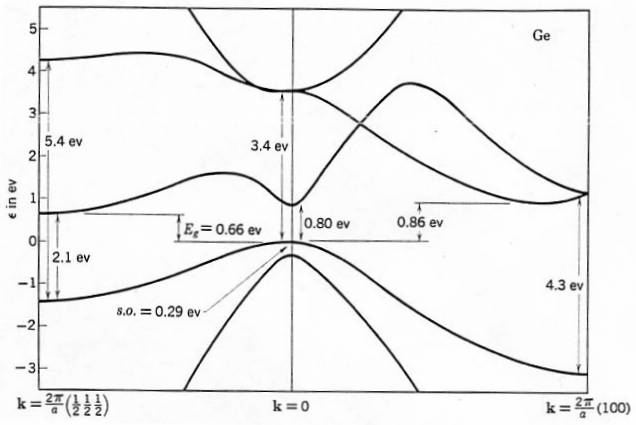
\includegraphics[width=0.4\textwidth]
{../Figuras/bandstructure.jpg}} 
\caption{\label{bandstructure}. Estructura de bandas del germanio tomado de~\cite{estructura de banda}}
\end{figure}

Acá se puede observar como el gap ha aumentado de una manera significativa desde el centro del diagrama hasta el nivel de 3.4$eV$, lo cual muestra que para llegar a ese punto se debe agregar mucha energía gracias a las propiedades de aislante mencionadas anteriormente.

\subsection{Efectos termoeléctricos}

Los efectos termoeléctricos que se trabajan en esta práctica son: El efecto Ettinghausen sucede al aplicar una corriente perpendicular al campo magnético sobre la muestra, un gradiente de temperatura perpendicular a ambas cantidades emerge. Como el efecto Hall, obliga a los portadores de carga a moverse perpendicular al campo y corriente aplicada, el número de colisiones aumenta en un lado calentando el material~\cite{Nernst}. Por otro lado, el efecto contrario, el efecto Nernst, al circular una corriente eléctrica en un campo magnético gracias a un gradiente de temperatura, se generará un campo eléctrico perpendicular a ambos. En este caso, se generará una decadencia en la resistencia Hall~\cite{Nernst}. Por último, el efecto Righic-Leduc, en el cual al aplicar un campo magnético a un flujo de calor establecido, un nuevo gradiente de temperatura, perpendicular a ambos aparecerá~\cite{Righic}. En este caso, se espera también una disminución con la resistencia Hall, dado el aumento de la temperatura.

\subsection{Resistencia Hall normal y en semiconductores}

Para poder definir la resistencia Hall, se necesita partir de las ecuaciones de movimiento las cuales son:

\begin{equation}
    v_x=-\frac{e\tau}{m}E_x - \frac{eB_z\tau}{m}v_y \\
\end{equation}

\begin{equation}
    v_y=-\frac{e\tau}{m}E_y + \frac{eB_z\tau}{m}v_x \\
\end{equation}

\begin{equation}
      v_z=-\frac{e\tau}{m}E_z
\end{equation}

Dónde en este caso, $e$ representa la carga del electrón; $\tau$ el tiempo característico de viaje; $m$, la masa del portador y $E_i$ y $B_z$ campos eléctricos y magnéticos asociados. En este caso, $E_x$ es el campo eléctrico horizontal que pasa por la figura y $E_y$, el campo eléctrico asociado al voltaje Hall. En todos los análisis realizados, el valor de $E_z$ siempre será 0.

Existen dos casos, cuándo suponemos que $v_y$ es 0, así:

\begin{equation*}
    E_y=B_zV_x 
\end{equation*}

Ahora, dado que hay una densidad de corriente $j_x$ solo en la dirección x (y definiendo $V_H=E_yd$), la resistencia Hall producida por una corriente circundante $I$, se define como 

\begin{equation}
  R_H=\frac{E_y}{j_xB_z}=\frac{V_Hw}{IB_z}
\end{equation}

Dónde $d$ es el alto de la placa y $w$, el ancho de esta.  Ahora al definir $j_x=-nev_x$, con $n$ siendo total de portadores de carga negativos\footnote{Esto también puede ser usado en portadores de carga positivo, conviertiendo $R_H=\frac{1}{pe}$}, el campo eléctrico de Hall se convierte en:
\begin{equation*}
    E_y=-\frac{B_zjx}{ne},
\end{equation*}

convirtiendo la ecuación 4 en:

\begin{equation}
    R_H=-\frac{1}{ne}
\end{equation}

El segundo caso es suponer que la velocidad en y es diferente de 0, pero la densidad de corriente en esta dirección es 0. Esto permite usar las ecuaciones 1 y 2 para encontrar que 

\begin{equation}
    R_H=\frac{ p\mu_h^2-n\mu_e^2}{e( p\mu_h+n\mu_e)},
\end{equation}

donde se define $\mu$ como la movilidad de los electrones y tiene la forma $\mu=\frac{e\tau}{m}$ para cada tipo de portador. Por último, se puede definir la conductividad como

\begin{equation*}
    \sigma=ne\mu_e + pe\mu_p,
\end{equation*}

lo que permite escribir la movilidad como 

\begin{equation}
    \mu=|R_H|\sigma
    \label{movilidad_hall}
\end{equation}

% trim={<left> <lower> <right> <upper>}
%----MONTAJE EXPERIMENTAL--------
\section{Montaje experimental}
\subsection{Instrumento de medición}

El montaje usado en esta práctica se presenta en la siguiente figura~\ref{montaje Hall}

\begin{figure}[h]
\center{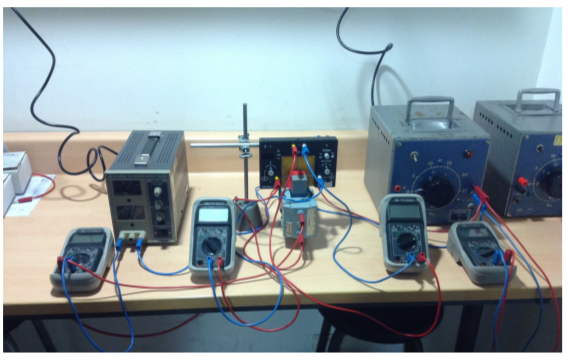
\includegraphics[width=0.4\textwidth]
{../Figuras/MontajeHall.PNG}} 
\caption{\label{montaje Hall}. Montaje para efecto Hall tomado de~\cite{guia hall}}
\end{figure}

Este montaje está constituido por una fuente de poder DC para las bobinas, una fuente de poder AC para el medidor de Hall; unos multímetros para monitorear los valores de $V_H$, el potencial horizontal, la corriente que pasa a través de las bobinas por la fuente DC y el valor de la fuente AC. El medidor de Hall se usa para medir la corriente y la temperatura que pasan de manera paralela por la muestra con dopaje P de germanio, mientras que las bobinas se utilizan para medir un campo magnético generado gracias a la corriente DC que pasa a través de estos. En la fuente AC, se debe mantener siempre un voltaje de 12 V, mientras que en la fuente DC se variará el valor de la corriente. Adicional a esto, hay un teslámetro utilizado en la primera parte para medir el campo magnético generado en las bobinas el cual se calibra para obtener una relación con la corriente que alimenta a estas.
%-----------------RESULTADOS----------------------
\section{Resultados y Análisis}
\subsection{Relación entre la corriente que pasa por el montaje y el campo magnético generado}
Dado que el Teslámetro que se tenía a disposición era un aparato sensible y delicado, se empezó primero por caracterizar como se comportaba el campo magnético generado por las bobinas en función de la corriente que circulaba por estas. Esto con el fin de que cuando se hablara de campo magnético, se supiera su equivalente en términos de la corriente y así con esto minimizar el uso del aparato.\\
Tal y como se muestra en la figura \ref{Calibracion}, la relación entre la corriente que circula por las bobinas y el campo magnético es de tipo lineal. Con esto se tiene entonces que hablar de corriente es equivalente a hablar de campo magnético\footnote{Es por esto que de ahora en adelante cuando se hable de campo magnético sus unidades serán Amperios}.

\begin{figure}[h]
\center{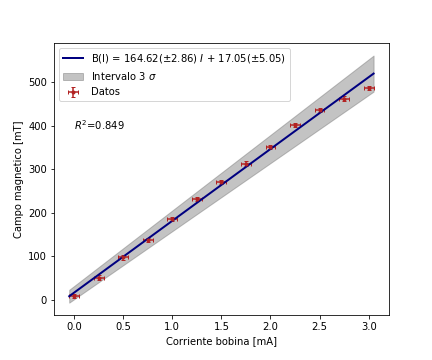
\includegraphics[width=0.4\textwidth]
{../Figuras/Calibracion_error.png}}
\caption{\label{Calibracion}. Gráfico del campo magnético medido por el Teslametro en función de la corriente suministrada por la fuente. La linea en azul corresponde al ajuste efectuado a los datos experimentales y la región sombreada corresponde a los intervalos de confidencia con $5\sigma$}
\end{figure}

\subsection{Determinación de la resistencia de Hall.}
Una vez caracterizado el campo magnético en función de la corriente, se fijó el campo magnético en 1.5 A y se analizó el comportamiento entre el voltaje de Hall $V_H$ en función de la corriente que pasaba por el material $I_p$.\\
Tal y como se muestra en la figura \ref{V_H_vs_I_p} se tiene que la relación entre estas dos cantidades es de tipo lineal y a partir de la regresión se tiene entonces que el valor de la resistencia de Hall es:
\[R_H=\frac{1.46\cdot 10^{-3}}{1.5(164.62)+17.05}\]
\[=5.53\times 10^{-3} (\pm 2.9\times 10^{-4}) \Omega\]
\begin{figure}[h!]
\center{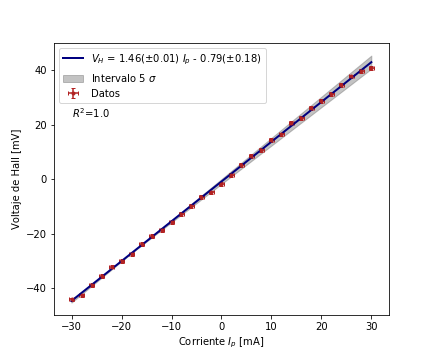
\includegraphics[width=0.4\textwidth]
{../Figuras/Voltaje_hall_ip.png}}
\caption{\label{V_H_vs_I_p}Voltaje de Hall en función de la corriente que atraviesa la placa de tipo $P$, Se observó una tendencia de tipo lineal para los datos experimentales. La linea en azul corresponde al ajuste efectuado a los datos experimentales y la región sombreada corresponde a los intervalos de confidencia con $5\sigma$}
\end{figure}

 De forma similar a la parte anterior se fijó el valor de la corriente $I_p$ en $-30 mA$ y luego se procedió a variar el campo magnético. En la figura \ref{V_H_vs_campo}  se observa el patrón obtenido; al igual que para la figura \ref{V_H_vs_I_p} se observó un comportamiento de tipo lineal, tal y como se esperaba, salvo que para este caso la linea formada tiene pendiente negativa, esto es explicado por el hecho de que la corriente que pasaba por la muestra tenía signo negativo.
\begin{figure}[h!]
\center{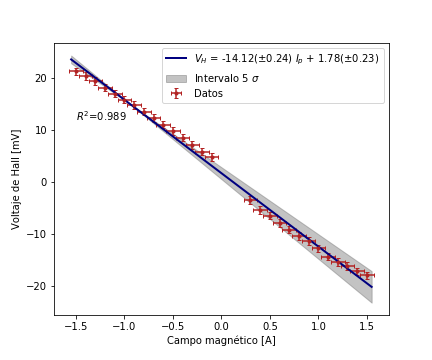
\includegraphics[width=0.4\textwidth]
{../Figuras/Voltaje_hall_Campo_magnetico.png}}
\caption{\label{V_H_vs_campo}Regresión del voltaje de Hall $V_H$ en función del campo magnético aplicado $B_z$.  La linea en azul corresponde al ajuste efectuado a los datos experimentales y la región sombreada corresponde a los intervalos de confidencia con $5\sigma$}
\end{figure}

A partir de la regresión mostrada en la figura \ref{V_H_vs_campo} se obtiene que la resistencia de Hall $R_H$ se puede calcular al regresar los valores de corriente a unidades de campo magnético por medio de la relación encontrada en la regresión de la figura \ref{Calibracion}, con lo cual se obtiene que:
\[R_H=\frac{0.1854}{30}\]
\[=6.18\times 10^{-3} (\pm 7.1\times 10^{-4})\Omega\]
Comparando con el resultado anterior se tiene que ambos valores obtenidos de $R_H$, se obtiene que la diferencia porcentual entre los valores obtenidos es de aproximadamente un $10\%$. Aunque es una diferencia bastante grande con respecto a lo esperado, se le atribuye esta discrepancia al hecho de la falta de control sobre el voltaje suministrado por la fuente $AC$, dado que esta aumentaba el voltaje que entregaba al circuito a medida que el tiempo pasaba. 
\subsection{Determinación de la resistencia longitudinal y su dependencia con el campo magnético}
En la figura \ref{V longitudinal vs ip} se muestra en resultado obtenido del comportamiento del voltaje longitudinal en función de la corriente que pasa por la muestra $I_p$ a campo cero. Como se puede observar también se presenta un carácter de tipo Ohmico con resistencia de $R_L = 55.17 (\pm 0.75)$
\begin{figure}[h!]
\center{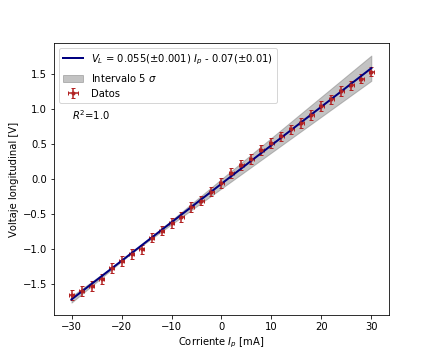
\includegraphics[width=0.4\textwidth]
{../Figuras/Voltaje_longitudinal_ip.png}}
\caption{\label{V longitudinal vs ip}Regresión del voltaje Longitudinal $V_L$ en función de la corriente que atravesaba la muestra $I_p$.  La linea en azul corresponde al ajuste efectuado a los datos experimentales y la región sombreada corresponde a los intervalos de confidencia con $5\sigma$}
\end{figure}

Una vez se caracterizó la resistencia longitudinal a campo nulo, se procedió a efectuar la misma toma de datos para diferentes valores de campo magnético ($0.25 - 3.0 A$) y se halló su respectivo ajuste para determinar el valor de la resistencia. Los resultados obtenidos de la resistencia relativa se muestran en la figura \ref{R_vs_Campo}. el resultado obtenido no corresponde a lo esperado (Un comportamiento de tipo cuadrático), esto parece atribuirse al hecho de que el circuito sobre el cual estaba montada la tarjeta parecía tener una falla, sin embargo, esto no se pudo comprobar dentro de los resultados obtenidos y por ende lo que se obtiene es que el comportamiento exhibido por la muestra tiene un comportamiento atípico con respecto al predicho por el efecto de magneto resistencia. Esto puede deberse al hecho de que durante esta toma de datos, la temperatura en la muestra estaba aumentando de manera extraña superando la temperatura ambiente, en la cual se debía hacer esta parte de la práctica.

\begin{figure}[h]
\center{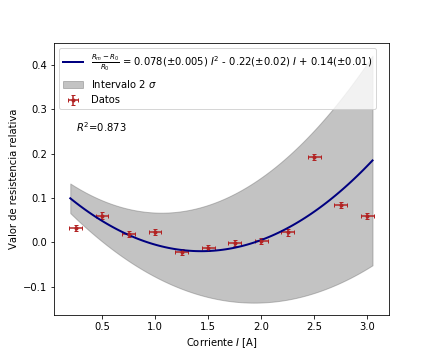
\includegraphics[width=0.4\textwidth]
{../Figuras/Resistencia_vs_Campo_magnetico.png}}
\caption{\label{R_vs_Campo}Ajuste de la resistencia relativa a la resistencia a campo cero en función del campo magnético aplicado.  La linea en azul corresponde al ajuste efectuado a los datos experimentales y la región sombreada corresponde a los intervalos de confidencia con $2\sigma$}
\end{figure}

\subsection{Efectos de la temperatura en la conductividad, el voltaje de Hall y la ``movilidad de Hall''}
A partir del modelo de conductividad en función de la temperatura para materiales semiconductores, se determinó la conductividad sobre el material como el inverso de la resistencia\footnote{Aunque la conductividad no es exactamente igual a el inverso de la resistencia, si se tiene una relación de proporcionalidad.}.

\begin{figure}[h!]
\center{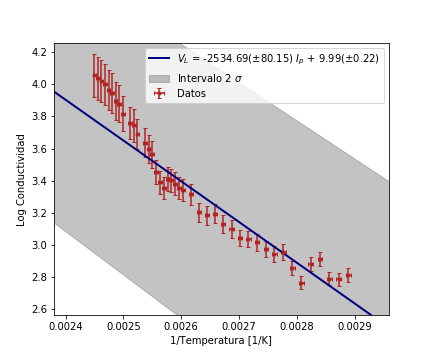
\includegraphics[width=0.4\textwidth]
{../Figuras/Comnductividad_Temperatura.png}}
\caption{\label{Conductividad en funcion de la temperatura}Gráfica del logaritmo de la conductividad en función del inverso de la temperatura.  La linea en azul corresponde al ajuste efectuado a los datos experimentales y la región sombreada corresponde a los intervalos de confidencia con $2\sigma$}
\end{figure}
En la figura \ref{Conductividad en funcion de la temperatura} se muestra un ajuste de tipo lineal a el logaritmo de la conductividad en función del inverso de la temperatura, a partir del ajuste se puede determinar el valor de la energía de GAP del material utilizado, con lo cual se obtuvo que esta energía tenia un valor de:
\[E_g=8.617\times 10^{-5}\cdot2534.69=0.218 (\pm 0.006) \ eV,\]
Comparando este resultado con el valor aceptado de energía para el Germanio\cite{Energia de gap}, se tiene que el resultado no está nada cerca de lo esperado, no obstante, dado que las fluctuaciones de la temperatura fueron tan altas, el resultado anterior no es de ``mucha'' confianza y se debe hacer un análisis adicional para comprobar esto. Con el fin de comprobar la veracidad del resultado anterior, se analizó el comportamiento del voltaje de Hall en función de la temperatura, los resultados obtenidos son mostrados en la figura~\ref{Region intrinseca}. A partir del ajuste efectuado y bajo la hipótesis que la concentración de portadores intrínsecos $n$  sigan la distribución de Maxwell-Boltzman, se tiene que el valor de la energía de GAP del material utilizado es:
\[E_g=2\cdot 3666.46 \cdot8.617\times 10^{-5}\]
\[=0.63 (\pm 0.02) eV,\]
lo cual corresponde al valor aceptado de energía de GAP para el Germanio \cite{Energia de gap}, presentando un error relativo del $4\%$. Con esto se concluye que la muestra con la que se está trabajando es de tipo semiconductora y dado el valor obtenido de energía de GAP, se tiene que la muestra está compuesta en su mayoría por Germanio.

\begin{figure}[h]
\center{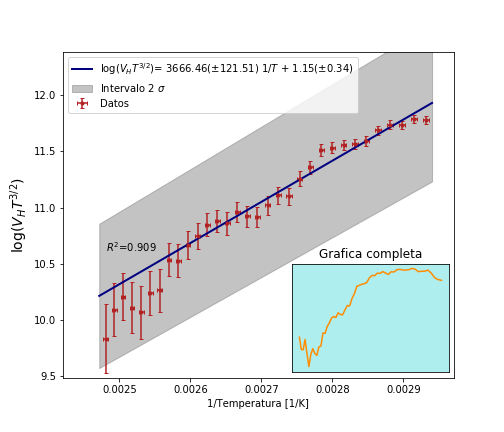
\includegraphics[width=0.4\textwidth]
{../Figuras/Region_intrinseca.png}}
\caption{\label{Region intrinseca}Gráfica del logaritmo del voltaje de Hall por la temperatura a los $3/2$ en función del inverso de la temperatura. En la gráfica se efectuó la regresión  sobre la región identificada como ``intrinseca'', la gráfica más pequeña muestra el comportamiento sobre todos los valores medidos de temperatura.}
\end{figure}


\begin{figure}[h!]
\center{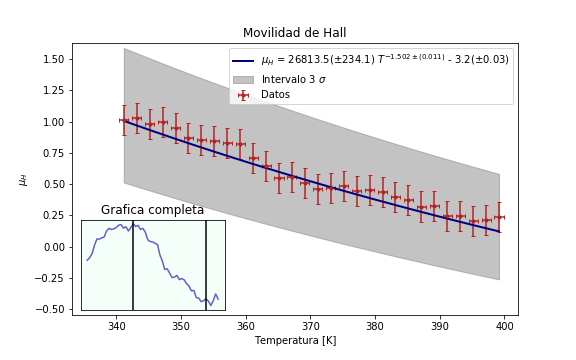
\includegraphics[width=0.4\textwidth]
{../Figuras/Movilidad_Hall.png}}
\caption{\label{movilidad de Hall}Gráfico de la movilidad de Hall en función de la temperatura, la gráfica pequeña muestra el comportamiento encontrado en las distintas temperaturas. La linea en azul corresponde al ajuste efectuado sobre la región descrita y la región sombreada corresponde a los intervalos de confidencia con $3\sigma$}
\end{figure}

Por ultimo se quiso verificar si existía una región en el cual el comportamiento de la movilidad de Hall descrito por la ecuación \eqref{movilidad_hall} estuviera descrito por un comportamiento de ley de potencias de la forma $T^{-3/2}$\footnote{Esto se puede deducir fácilmente del hecho de que $R_H\sim T^{-3/2}e^{E/K_BT}$ y $\sigma \sim e^{E/K_BT}$, así de esta forma se deduce que el comportamiento para esta región será $\propto T^{-3/2}$}. En la figura \ref{movilidad de Hall} se muestra el comportamiento encontrado en función de la temperatura. Tal y como se esperaba se encontró una región sobre la cual este se exhibe un comportamiento de ley de potencias ( Región entre los $330$ y los $410 K$), al encontrar que el exponente es $-1.502 (\pm 0.011)$ se deduce que esta región es la región en la que dominan procesos de dispersión de fonones.
%---------------CONCLUSIONES-------------------

\section{Conclusiones}
\begin{itemize}
    \item Gracias a las figuras~\ref{V_H_vs_I_p} y \ref{V_H_vs_campo} se puede decir que se observa el efecto Hall para placas tipo P con éxito gracias a la cercanía entre sus coeficientes Hall, que en este caso tiene una discrepancia del 10\% gracias los súbitos cambios de voltaje y corriente que proporcionaba la fuente que alimentaba al medidor de Hall. No obstante, gracias al comportamiento lineal de ambas gráficas, se puede afirmar que para ambos se obtiene el comportamiento deseado (lineal) reiterando lo dicho al comienzo del párrafo.
    \item Al observar la figura~\ref{R_vs_Campo} se puede afirmar que no se vio con éxito el comportamiento esperado, esto se puede deber principalmente a los repentinos saltos de temperatura en esta toma de datos, los cuales siempre tuvieron un comportamiento lineal, lo cual va de la mano con lo visto en las figuras anteriores a esta. Con respecto a la temperatura (figuras~\ref{Conductividad en funcion de la temperatura} y \ref{Region intrinseca}) 
    \item Observando la figura~\ref{V_H_vs_campo} se nota que al cambiar la dirección de corriente se obtiene un cambio en la pendiente. Esto indica un comportamiento positivo de la tarjeta de tipo (dada la orientación con la corriente) esto tiene sentido pues como se ve en la literatura, un dopaje tipo P aumenta la banda aislante, aumentando los portadores de carga positivos. Y con la figura , se puede observar que en la densidad de partículas
\end{itemize}
%Se deben contestar las preguntas planteadas inicialmente o dar las razones por las cuales no es posible hacerlo. Las conclusiones deben ser necesariamente una consecuencia del experimento realizado, es decir que no se deben tocar aspectos que no se hayan expuesto en la sección de resultados y análisis. Si escribe algo que no se encuentra en la sección de resultados y análisis, esto quiere decir que hace falta incluir material en resultados y análisis. Concluir únicamente aspectos pertinentes a su trabajo en el laboratorio; evite generalizaciones que no hablan concretamente de lo que usted hizo o midió.

\begin{thebibliography}{9}

\bibitem{Efecto Hall}
Woodford, c. \textit{Hall Effect Sensors}, \textit{Explain that stuff}, 2018 \url{https://www.explainthatstuff.com/hall-effect-sensors.html}
\bibitem{Klitzing}
 K. v. Klitzing, G. Dorda, and M. Pepper. \textit{New method for high-accuracy determination of thefine-structure constant based on quantized hall resistance}.Phys. Rev. Lett., 45:494–497, Aug 198
\bibitem{doping}
Laube, P; \textit{Semiconductor technology from A to Z}.\url{https://www.halbleiter.org/en/fundamentals/doping/}
\bibitem{estructura de banda}
\url{http://www.globalsino.com/micro/1/1micro9970.html}
\bibitem{Nernst}
 Ettingshausen, A.; Nernst, W. (1886). \textit{Ueber das Auftreten electromotorischer Kräfte in Metallplatten, welche von einem Wärmestrome durchflossen werden und sich im magnetischen Felde befinden}. Annalen der Physik und Chemie. 265 (10): 343–347.
 \bibitem{Righic}
 Qing-Lian Xu, Zhen-Gang Zhu, Gang Su, \textit{Generalized Fourier law and anomalous Righi–Leduc effect in a ferromagnet}, Physics Letters A, Volume 382, Issues 42–43, 2018,Pages 3115-3119, ISSN 0375-9601, https://doi.org/10.1016/j.physleta.2018.08.006. \url{(http://www.sciencedirect.com/science/article/pii/S0375960118308648)}
 \bibitem{guia hall}
 Mejía, J; Universidad de los Andes. \textit{Efecto Hall}, 2017.
\bibitem{Energia de gap}
\url{http://www.ioffe.ru/SVA/NSM/Semicond/Ge/bandstr.html}
\end{thebibliography}

\end{document}
%
% ****** End of file apssamp.tex ******

